\documentclass[a4paper]{article}
\usepackage[UTF8]{ctex}
\usepackage{geometry}
\usepackage{graphicx}
\usepackage{url}
\usepackage{multirow}
\usepackage{array}
\usepackage{booktabs}
\usepackage{url}
\usepackage{enumitem}
\usepackage{graphicx}
\usepackage{float}
\usepackage{amssymb}
\usepackage{amsmath}
\usepackage{subfig}
\usepackage{longtable}
\usepackage{pifont}
\usepackage{color}
\usepackage{listings}
\usepackage{xcolor}

\allowdisplaybreaks

\geometry{a4paper, scale=0.78}

% \begin{figure}[H]
%     \centering
%     \includegraphics[width=.55\textwidth]{E.png}
%     \caption{矩阵与列向量的乘法}
%     \label{fig:my_label_1}
% \end{figure}

% \left\{
% \begin{array}{ll}
%       x+2x+z=2 & \\
%       3x+8y+z=12 & \\
%       4y+z=2
% \end{array}
% \right.

% \begin{enumerate}[itemindent = 1em, itemsep = 0.4pt, parsep=0.5pt, topsep = 0.5pt]

% \end{enumerate}

%\stackrel{a}{\longrightarrow}

\title{Probability Graph 06 Inference Background}
\author{Chen Gong}
\date{28 November 2019}

\begin{document}
\maketitle
推断(Inference)这个词,对于有一定机器学习基础的同学来说,一定是听说过,这也是贝叶斯方法中一个非常重要的理论性研究。那么什么是推断呢?推断说白了,就是求概率。比如,对于一个联合概率密度函数$p(x)=p(x_1,x_2,\cdots,x_p)$。我们需要求的有哪些呢?

1. 边缘概率:$p(x_i) = \sum_{x_1}\cdots\sum_{x_{i-1}}\cdots\sum_{x_{i+1}}\cdots\sum_{x_p}p(x)$。

2. 条件概率:$p(x_A|x_B)$,令$x=x_A\cup x_B$。

3. MAP Inference:也就是$\hat{z} = \arg\max_z\ p(z|x) \varpropto \arg\max \ p(x,z)$。因为$p(z|x) = \frac{p(x,z)}{p(x)} \varpropto p(x,z)$,我们的目标是求一个最优的参数$z$,并不需要知道具体的数值是多少,只要知道谁大谁小就行,所以$p(x)$可以直接不看了。

现在我们知道了,Inference在求什么?下一步,我们要总结Inference有哪些方法。

\section{Inference求解方法}
\subsection{精准推断(Deterministic Inference)}
Variable Elimination (VE),变量消除法;Belief Propagation (BP)信念传播,这个可不是我们之前学习的反向传播算法,这里需要注意。同时这个算法衍生出的Sum Product Algorithm,这就是推断的核心,这是一种树结构的;而Junction Tree Algorithm,这是一种普通图结构。

\subsection{近似推断(Approximate Inference)}
典型的有有向环(Loop Belief Propagation);采样方法,包括Mente Carlo Inference:Importance Sampling,MCMC;最后一个就是我现在主要研究的变分推断(Variational Inference)。

\section{隐马尔可夫模型(Hidden Markov Model)}
Hidden Markov Model (HMM)算法将在后面的章节中做详细的描述,在这一小节中,我们主要
\begin{figure}[H]
    \centering
    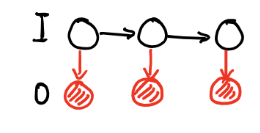
\includegraphics[width=.3\textwidth]{微信图片_20191128115946.png}
    \caption{HMM的模型结构}
    \label{fig:my_label_1}
\end{figure}
做一点概述性的描述。HMM的模型可视化为上图所示,其中$O$是隐变量,也就是我们的观测变量。

我们主要考虑三个问题,在三个问题为Inference的问题。1. Evaluation,也就是求一个边缘密度$p(O) = \sum_I P(I,O)$。2. Learning,也就是寻找$\hat{\lambda}$。3. Decoding:$\hat{I} = \arg\max_I P(I|O)$,包括Vitebi Algorithm,这是一个动态规划算法。而隐马尔可夫模型实际上一种动态规划模型(Dynamic Bayesian Network)。














\end{document}
